\section{Arquitectura del tp2}


RELACIONAR ARQUITECTURA CON ATRIBUTOS DE CALIDAD ANTERIORES

Para empezar, se presenta la arquitectura correspondiente al Tp2.\newline

\subsection{General}

Tenemos dos formas de observar nuestra arquitectura, la primera con un enfoque general donde se ven
los componentes externos a nuestro sistema que interactuan con nosotros. Con 
esta vision, nuestra arquitectura se ve como un único componente monolitico pues es mas sencillo a
este nivel, sin embargo, contamos con una arquitectura distribuida a lo largo y ancho del país 
que podremos ver con mas detalle en las siguientes vistas.

\begin{figure}
\centerline{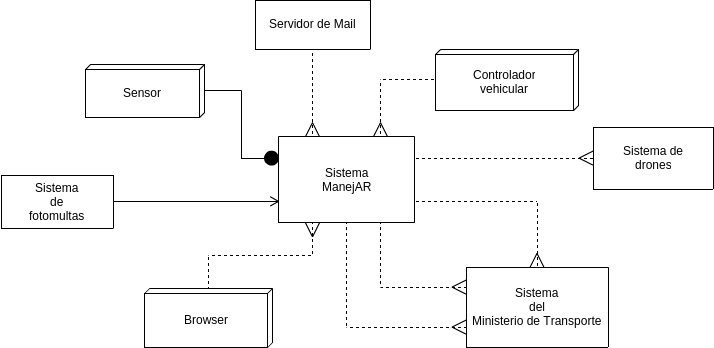
\includegraphics[width=1\textwidth]{./imagenes/arquitectura_tp2/general.png}}
\caption{Arquitectura general}
\end{figure}

Como podemos ver, son varios los componentes externos que interactuan con 
nuestro sistema, cada uno con sus particularidades que pasaremos a detallar.

\subsection{Sensor}
Los \textbf{sensores} son nuestros dispositivos ubicados a lo largo del país, sobre todo en La 
Pampa, que utilizamos para medir la conectividad de la zona.
En estos dispositivos, distinguimos dos componentes claves para describir la 
arquitectura.

\begin{itemize}
  \item Receptor de mediciones de conectividad: Recolecta las mediciones del 
  hardware y las encola en el proximo componente.
  
  \item Comunicador con administrador de sensores: Toma las mediciones y las 
  envia al Administrador de sensores de nuestro sistema \textbf{ManejAR}.
  \end{itemize}


La particularidad de la conexion entre este ultimo componente y el sistema 
manejar es que el medio tiene perdida de paquetes pero decidimos no crear una 
estrategia de reenvio pues enviamos esas mediciones cada 5 segundos.


\begin{figure}
\centerline{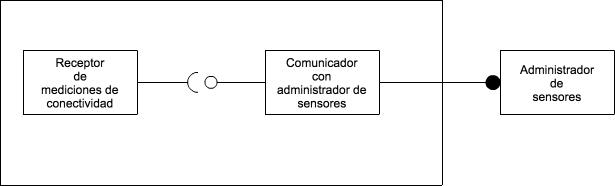
\includegraphics[width=1\textwidth]{./imagenes/arquitectura_tp2/sensor.png}}
\caption{Arquitectura interna de los Sensores}
\end{figure}

\subsection{Control Vehicular}
El controlador vehicular, es el componente que se encuentra en cada uno de los vehiculos que deben
ser monitoreados. En este componente encontramos los siguientes subcomponentes.

Receptor de mediciones: Este se encarga de recibir las mediciones realizadas por el GPS de su vehiculo,
 y las guarda en un repositorio de Mediciones.
 
Mediciones: Es el repositorio donde se almacenan las mediciones del GPS.
 Es importante la presencia de este componente de almacenamiento, porque nos permite preservar
las mediciones hasta que hayan sido enviadas, fundamental para no perder mediciones ante un
 problema de conectividad.
Transmitidor: Encargado de asegurarse del envio de las mediciones al Balanceador, del Sistema Manejar.
Antes de enviar cualquier dato, se comunica con el Encriptador y el Checksum para proteger la
integridad y confidencialidad de los datos. Cada medicion enviada exitosamente sera borrada del
repositorio Mediciones. En caso de no disponer de conectividad, se reintentara el envio de la medicion
cuando logre conectarse. De esta manera nos aseguramos no perder mediciones, y
 contar con todas las mediciones generadas.

\begin{figure}
\centerline{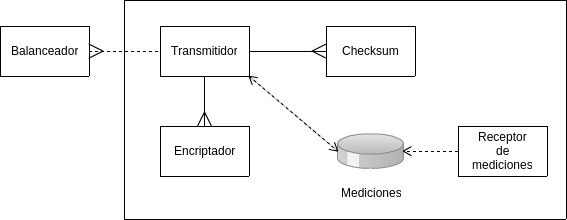
\includegraphics[width=1\textwidth]{./imagenes/arquitectura_tp2/controlador_vehicular.png}}
\caption{Arquitectura interna de los Controladores vehiculares}
\end{figure}


\subsection{Sistema Manejar}

Si nos concntramos en los componentes dentro del cuadro blanco, podemos 
organizarlos en dos categorias [[NOTA: Esto es la vista de deploy ]]

* Esta en servidor central
* Distribuido en diferentes nodos a lo largo del pais.

El \textit{Controlador de datos de GPS} y el \textit{Administrador de Base de Datos} 
son los únicos que estan distribuidos en todos los nodos a lo largo del país, 
con el objetivo de optimizar el procesamiento de datos y a su vez, asegurar la 
disponibilidad del servicio ya sea del procesamiento como la redundancia de las bases de datos.


\begin{figure}
\centerline{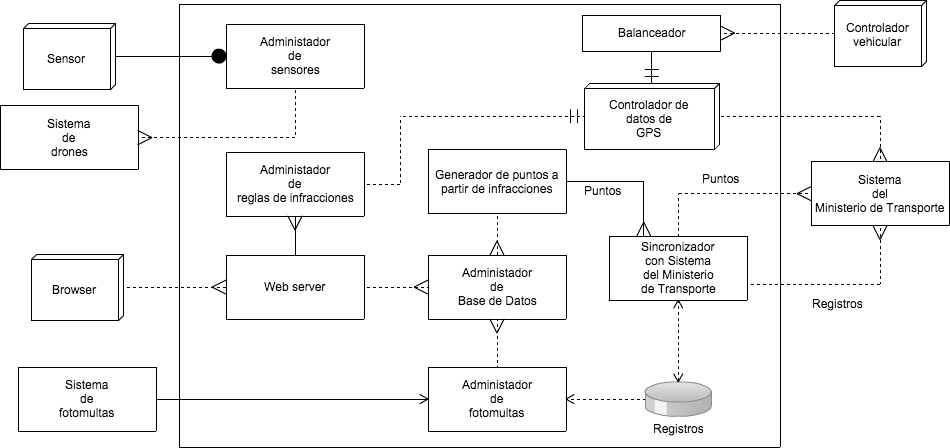
\includegraphics[width=1\textwidth]{./imagenes/arquitectura_tp2/manejar.png}}
\caption{Arquitectura interna del Sistema ManejAR}
\end{figure}

La mayoría de estos componentes los explicaremos en detalle más adelante con su 
respectiva vista. Para los que no, alcanza la siguiente descripción de los 
mismos.


\subsubsection{Administrador de reglas de infracciones}

Es el encargado de recibir las modificaciones en las reglas de infracciones y 
notificarlas a todos los \textbf{Controladores de datos de GPS} usando un \textit{broadcast}.

\subsubsection{Generador de Puntos a partir de Infracciones}

Todas las noches este componente toma las infracciones del \textbf{Administrador de Bases de Datos} 
y calcula el puntaje a restar a cada conductor. Luego se lo informa al
\textbf{Sincronizador con Sistema del Ministerio de Transporte}.

\subsubsection{Sincronizador con Sistema del Ministerio de Transporte}

Las responsabilidades de este componente son dos.
La primera es actualizar nuestra base de registros directamente del \textbf{Sistema del Ministerio de Transporte}
para poder identificar los conductores profesionales de los particulares. 
La segunda envia los puntos a descontar a cada conductor profesional.

\subsubsection{Balanceador}
El balanceo de carga es un concepto usado que se refiere a la técnica usada para compartir el trabajo
a realizar entre varios procesos, ordenadores, discos u otros recursos.
El balanceo de carga se mantiene gracias a un algoritmo que divide de la manera más equitativa posible
el trabajo, para evitar los así denominados cuellos de botella y mantener una 
alta performance y disponibilidad del sistema.


\subsection{Controlador de datos de GPS}

\begin{figure}
\centerline{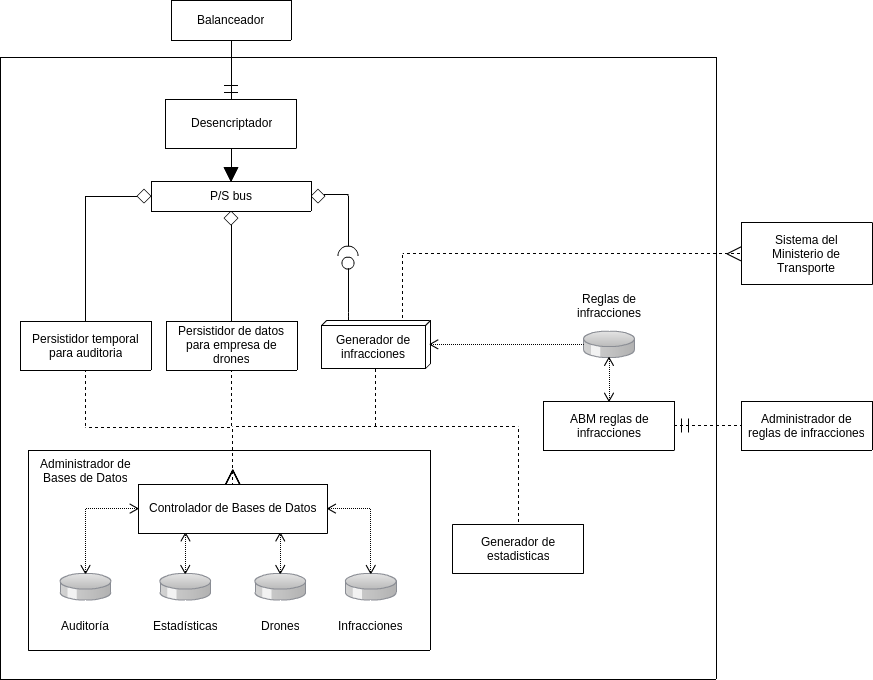
\includegraphics[width=1\textwidth]{./imagenes/arquitectura_tp2/controlador_datos_gps.png}}
\caption{Arquitectura interna del Controlador de datos de GPS del Sistema ManejAR}
\end{figure}


\subsection{Administrador de Fotomultas}



\begin{figure}
\centerline{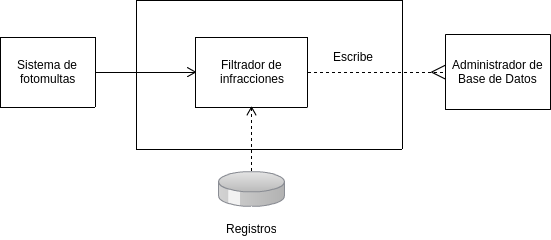
\includegraphics[width=1\textwidth]{./imagenes/arquitectura_tp2/administrador_fotomultas.png}}
\caption{Arquitectura interna del Administrador de Fotomultas del Sistema ManejAR}
\end{figure}


\subsection{

\begin{figure}
\centerline{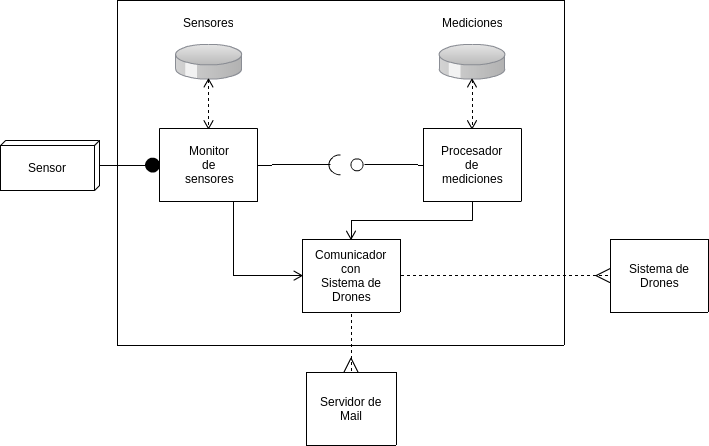
\includegraphics[width=1\textwidth]{./imagenes/arquitectura_tp2/administrador_sensores.png}}
\caption{Arquitectura interna del Administrador de Sensores del Sistema ManejAR}
\end{figure}


\begin{figure}
\centerline{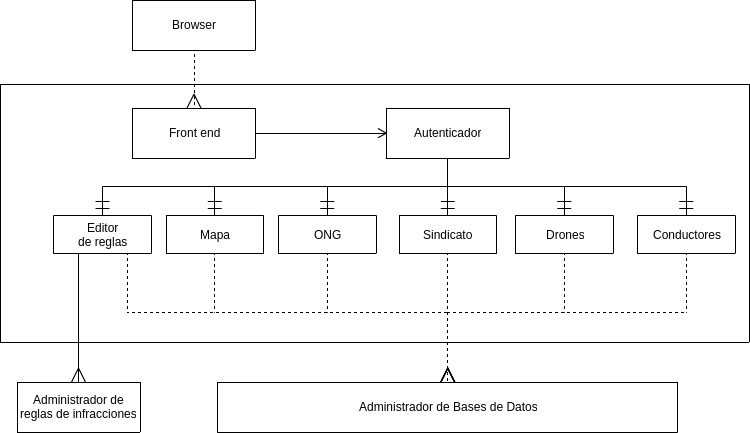
\includegraphics[width=1\textwidth]{./imagenes/arquitectura_tp2/web_server.png}}
\caption{Arquitectura interna del Web Server del Sistema ManejAR}
\end{figure}
